
\chapter[A Proposta]{A PROPOSTA}

A proposta deste trabalho é criar uma ferramenta capaz de produzir projetos de gamificação, a ferramenta servirá para automatizar o processo de criação dos projetos, simplificar e incentivar a inserção de gamificação no cotidiano das pessoas que tem interesse pelo tema e querem aplicá-lo as suas vidas. Este capítulo está estruturado da seguinte maneira: introdução, onde será feita uma contextualização sobre o porque de se construir uma ferramenta com tal propósito, construção da ferramenta, onde será descrito o processo de construção da ferramenta.

\section{Introdução}


Proposta do projeto - Porque a ferramenta tem que existir?
Porque ela é necessária? Qual a motivação? Porque é importante?

Estágio 1. Estabelece um contexto que ajuda os leitores a entenderem como a
pesquisa se situa num campo de estudo maior
Estágio 2. É feita uma revisão bibliográfica, ou seja, são apresentados aspectos do
problema que já foram estudados por outros pesquisadores.
Estágio 3. Indica a necessidade de mais investigação na área
Estágio 4. Indica os objetivos/propósitos do estudo
Estágio 7. (opcional) Dá uma justificativa para se empreender o estudo em questão,
afirmando o valor do trabalho
Estágio 8. (opcional) Define a estrutura do trabalho, isto é, seu outline


Gamificação é um tema Para motivar o ser humano, gamificação é um novo olhar sobre motivação e como motivar pessoas, vai além de inserir elementos de jogos em contextos fora de jogos, gamificar é trazer pra vida real o incentivo natural que se tem ao jogar jogar um jogo, ao tentar conquistar a vitória no jogo. Há algumas décadas têm-se estudado a motivação intrinsecamente ligada ao jogo e como aplicá-la em outras áreas com o mesmo sucesso. Mas motivar apenas não basta, motivação acaba, é preciso pensar maneiras de manter a motivação, criar um ciclo onde além de motivadas as pessoas permaneçam disciplinadas, mas não por obrigação, e sim porque sentem vontade de sempre seguir adiante.

Apesar da ascenção do tema na última década ainda não existem maneiras simples de criar uma gamificação, existem menos ainda maneiras simples de criar uma gamificação efetiva, que motive o usuário do início ao fim e o auxilie a  conquistar uma meta de maneira disciplinada e divertida e que não pareça uma obrigação.

Para que o nivel de conhecimento exigido atualmente para se criar uma gamificação seja diminuído. A pessoa não vai precisar estudar o framework do Yu-Kai Chou para conseguir montar uma simplificação.

Para aumentar a produtividade de usuários com grau de conhecimento sobre gamificação.

Para relacionar os cores do octalysis e descobrir quais cores funcionar melhor em conjunto.

Para relacionar as técnicas da mesma maneira que os cores foram relacionados, e identificar quais podem interagir com quais e quais devem ser evitadas.

Para melhorar a usabilidade da plataforma

Para dar origem a funifier store 
A atividade que proporciona prazer e felicidade não é a mesma para todas as pessoas, e ela pode acontecer de forma casual, através de uma combinação de fatores internos e externos. A execução de atividades que produzem a sensação de prazer oferece também ao indivíduo a sensação de descoberta. É neste crescimento contínuo da personalidade que está um dos segredos para o alcance do momento flow (TED, Mihaly Csikszentmihaly, 2014).

Apesar de ser uma ferramenta para construção de gamificações e não uma ferramenta gamificada a inserçação de dados e o seu comportamento deve ser leve e fluído, de fácil uso  e interação por parte do usuário, para que não tenha os mesmos problemas encontrados na inserção de dados feitos através das planilhas excel e não desmotive o usuário logo no inicio do processo de construção da gamificação. E porque seria contraditório construir uma ferramenta massante e arcaica dentro de um contexto de gamificação, seria iniciar todo o processo comentendo um erro.


Segundo Yu-Kai Chou \cite{arruda2007} gamificação é o ato de cuidadosamente aplicar ao mundo real e as atividades produtivas os elementos divertidos e envolventes dos jogos, o que torna o ato de gamificar mais complexo que apenas incorporar elementos de jogos em outros contextos, gamificar é mais sobre  motivar pessoas e menos sobre pontos e troféus. 

Para produzir motivação através de gamificação Chou criou o Octalysis framework, composto de oito unidades principais, cada unidade principal possui um número variável de técnicas, as técnicas de gamificação compõem internamente as unidades principais e servem de suporte para os aspectos que pretende-se motivar. As técnicas incorporam elementos de jogos para conduzir a motivação e para que as unidades principais sejam implementadas corretamente não é necessário fazer uso de todas as técnicas.
\newpage

\section{Construção da ferramenta}

A figura X representa os componentes internos que serão utilizados para dar forma a ferramenta, cada cubo da figura representa os cores drives, técnicas de gamificação e os atributos das técnicas de gamificação. Os cores drives, representados como a parte superior do cubo, são as unidades principais do framework e serão também o principal componente da ferramenta, as técnicas de gamificação, representadas como o lado esquerdo do cubo, compõem as unidades principais, os atributos, representados como o lado direito do cubo, compõem as técnicas de gamificação. Como a ferramenta tem como propósito da construção de projetos gamificação que motivem os seus usuários ela terá o usuário como foco principal, como indicado na figura, o design focado no ser humano \cite{Chou2014} ou design centrado no usuário \cite{JanakiMythilyKumar and Mario Herger}, indica que o processo de concepção e desenvolvimento da gamificação será focado no usuário e nas suas motivações. 

\begin{figure}[h]
	\centering
	\label{fig01}
		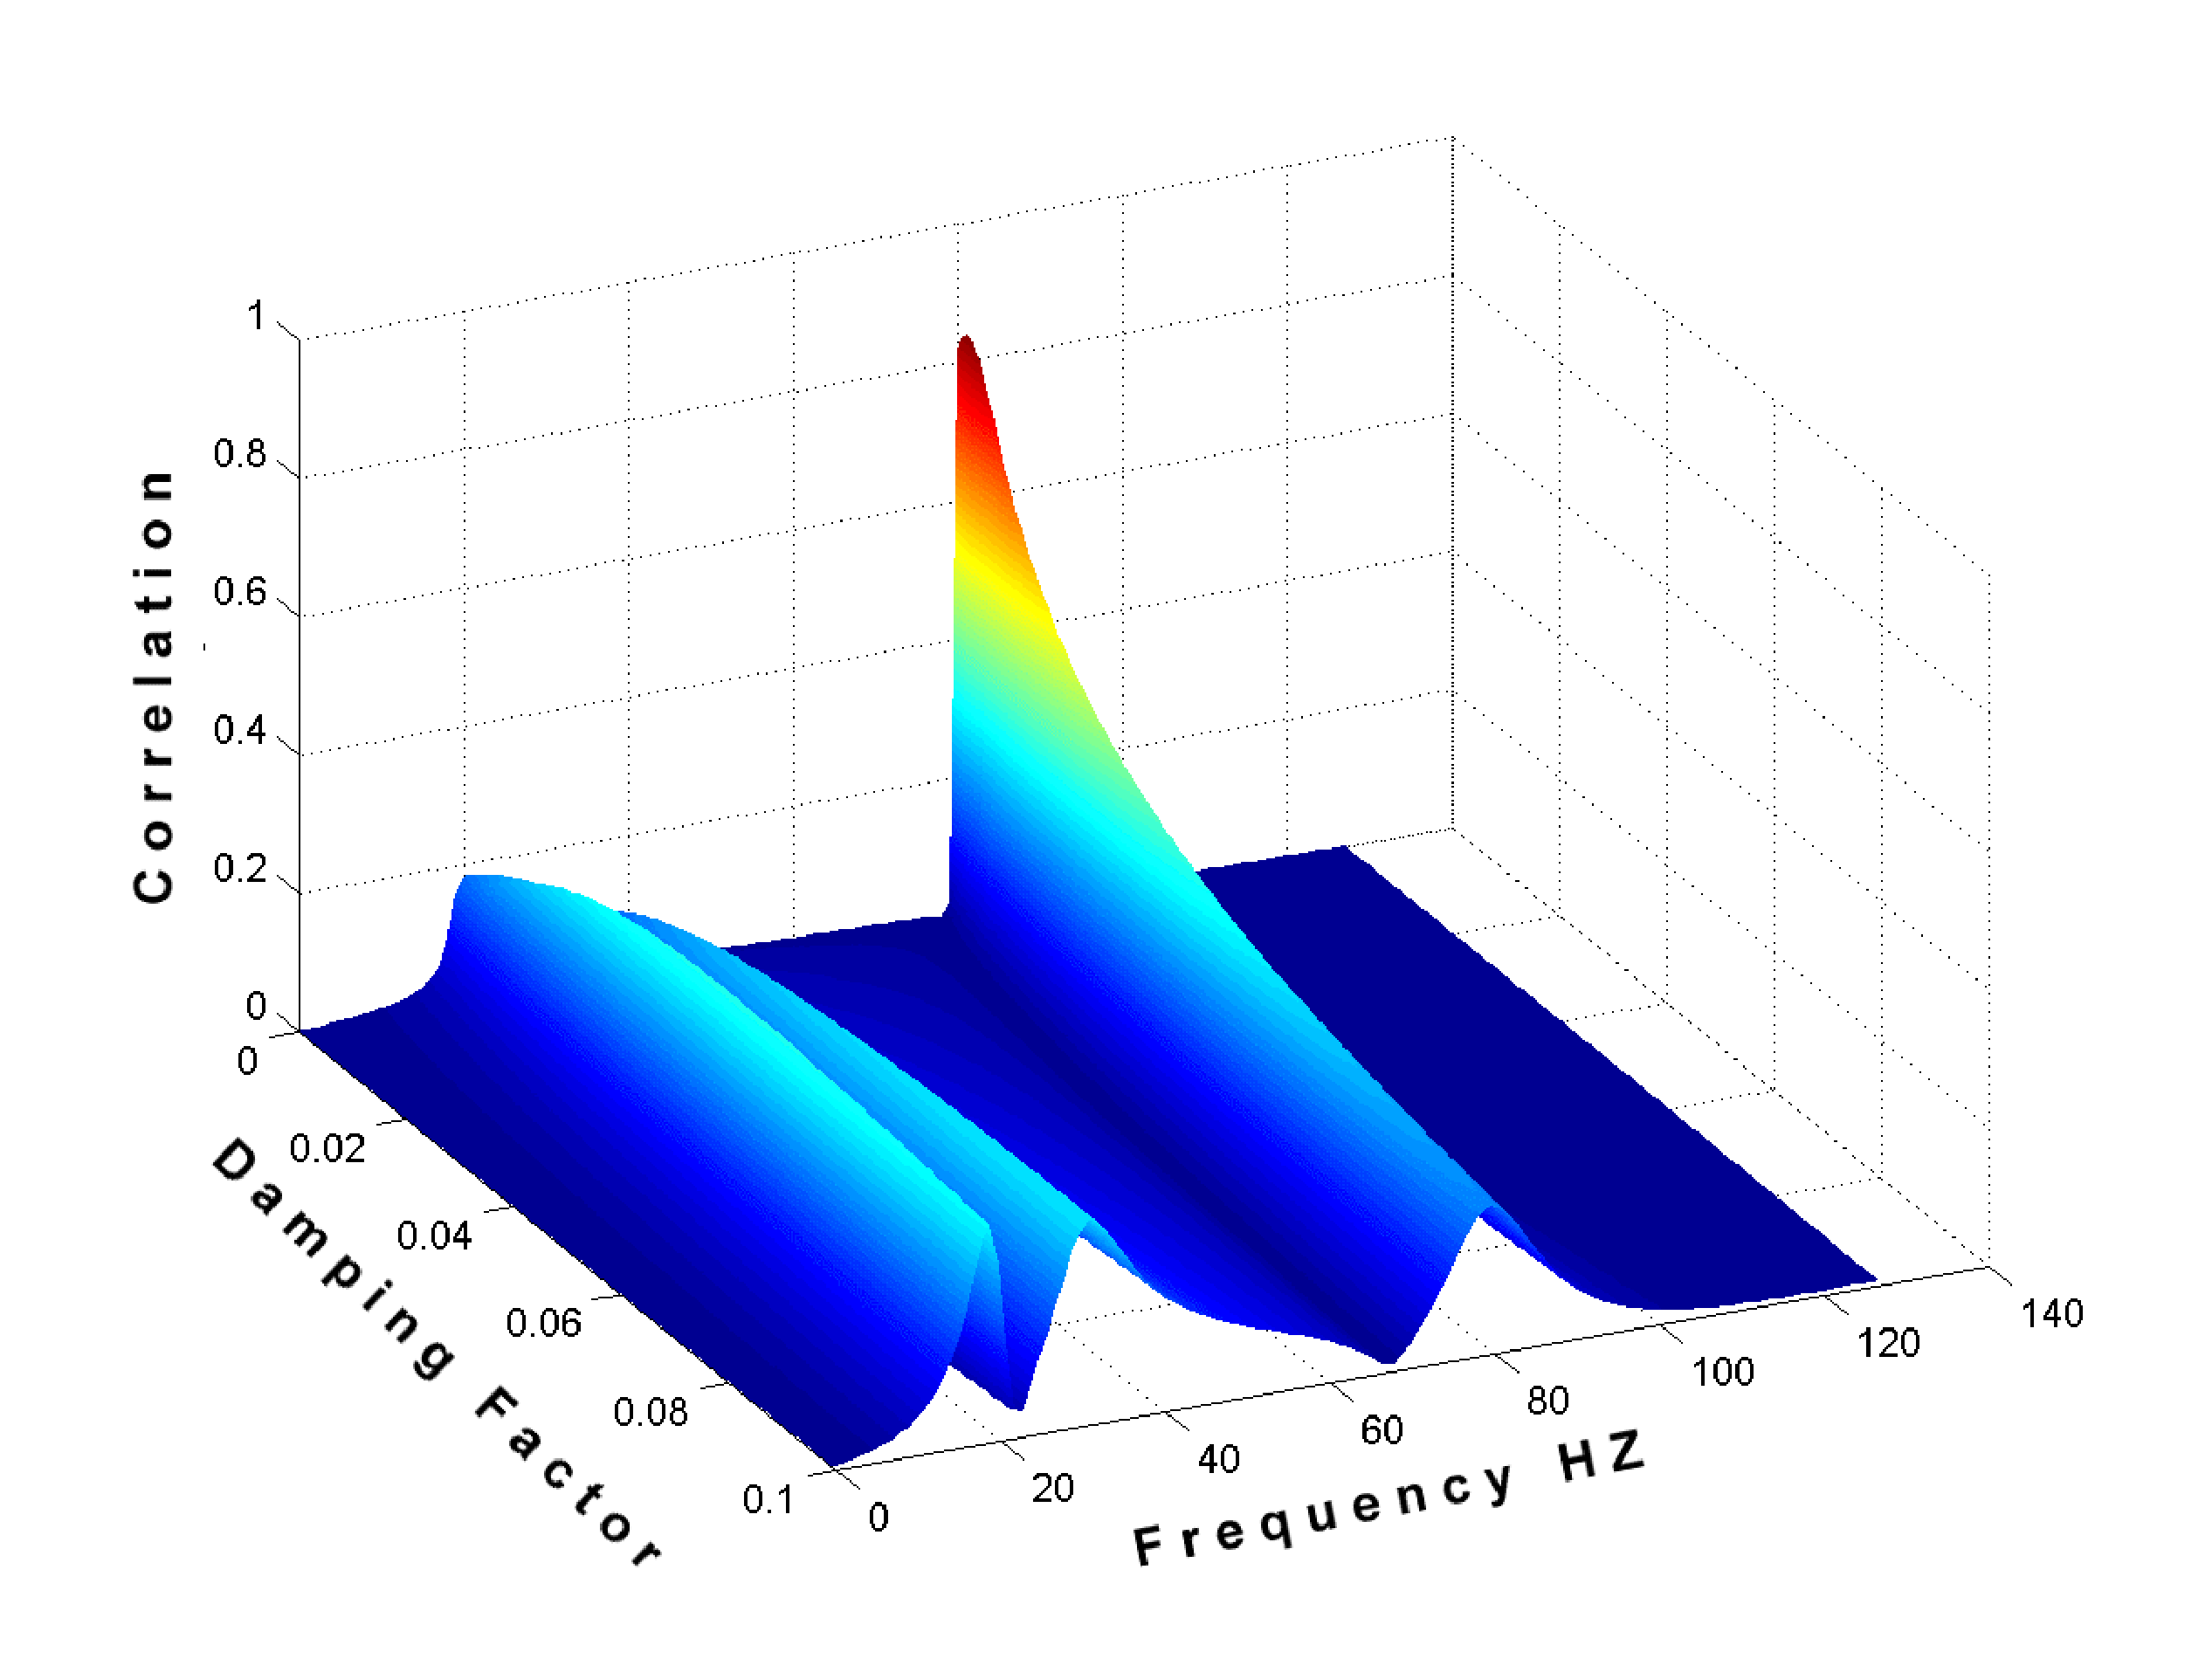
\includegraphics[keepaspectratio=true,scale=0.3]{figuras/fig01.eps}
	\caption{Wavelets correlation coefficients}
\end{figure}

Para que a ferramenta possa ser construída de maneira adequada e que proporcione ao usuário uma experiência bem sucedida na criação do seu projeto de gamificação, o framework octalysis foi escolhido como alicerce para a construção da mesma, as unidades principais do framework juntamente com as técnicas de gamificação existentes estão bem alinhadas com o principal próposito da ferramenta. Yukai-Chou utiliza as unidades principais do framework para motivar os usuários, e as técnicas de gamificação para representar elementos de jogos, mas as técnicas possuem mais de uma função, elas são utilizadas também para intensificar a motivação representada pela unidade principal da qual fazem parte. O emprego correto das mesmas na construção do projeto de gamificação produz um resultado mais satisfatório. Para que uma gamificação produza um bom resultado as técnicas de gamificação devem ser utilizadas de maneira a se complementarem, atualmente não há uma definição formal de um conjunto mínimo de atributos que devem estar presentes para que uma técnica seja implementada corretamente e não há um mapeamento que informe ao construtor do projeto de gamificação como as técnicas se relacionam, se é possível implementar todas de uma vez, se a implementação de uma afeta a implementação de outra, não há uma definição de como deve ser o relacionamento entre as técnicas de gamificação e isso acarreta uma dificuldade para identificar se o projeto de gamificação está sendo construído corretamente. As oito unidades principais do octalysis possuem uma descrição e são compostas por inúmeras técnicas de gamificação, já as técnicas de gamificação possuem uma descrição, mas não é especficado qual a sua composição, para construir a ferramenta definiu-se então um conjunto de atributos que compõem as técnicas e será realizado um mapeamento que indicará se há relacionamento entre as técnicas e como isso influencia na construção do projeto de gamificação.  

O conjunto de atributos definidos para compor a estrutura interna das técnicas são alguns dos indicadores de engajamento definidos por \cite{fredericks2004}, Fredericks divide os engajamentos em três tipos, o engajamento emocional, que trata, por exemplo, de emoções como alegria, interesse e raiva, o engajamento comportamental, que trata de indicadores de conduta, tais como, esforço, atenção e persistência e o engajamento congnitivo, que trata, por exemplo, de flexibilidade para resolver um problema, concentração e domínio. Engajamento também pode ser interpretado neste contexto como envolvimento, cada tipo de engajamento possui alguns indicadores, os indicadores caracterizam os tipos de engajamento e foram escolhidos aqui também para caracterizar as técnicas de gamificação, tal como se fossem adjetivos caracterizando as técnicas de gamificação.  A estrutura interna das técnicas é igual, independente da técnica de gamificação em questão. Os indicadores escolhidos para compor a estrutura interna das técnicas são: 

\begin{itemize}
\item  \textbf {Envolvimento com o trabalho:}  Mensura a quantidade de envolvimento com a gamificação que a técnica exigirá do usuário.
\item  \textbf {Participação:}  Mensura quanta participação efetiva na gamificação a técnica exigirá do usuário
\item  \textbf {Atenção:}  Mensura quanta atenção a gamificação exigirá do usuário.
\item  \textbf {Persistência:} Mensura quão persistente o usuário será para obter resultados no projeto de gamificação. 
\item  \textbf {Domínio:} Mensura a quantidade de maestria que o usuário precisará dispor para executar a técnica de gamificação. 
\item  \textbf{Social:} Mensura a quantidade de envolvimento social que a técnica dispõe para o usuário e quão social a técnica pode ser.
\end{itemize}


Cada indicador representará um atributo da técnica de gamificação e receberá uma valor que representa o grau de pertinência à técnica de gamificação, os valores variam de um a cinco e serão concedidos de acordo com a escala de Likert. A escala de Likert  \cite{arruda200} utilizada possui cinco itens: 

\begin{itemize}
\item  \textbf {1 - Muito aquém:} O atributo influência fracamente a técnica de gamificação
\item  \textbf {2 - Aquém:} O atributo influencia aquém do normal a técnica de gamificação
\item  \textbf {3 - Suficiente / Normal:} O atributo influencia de forma suficiente (normal) a técnica de gamificação
\item  \textbf {4 - Além:} O atributo influência além da normal a técnica de gamificação
\item  \textbf {5 - Muito além:} O atributo influencia plenamente a técnica de gamificação
\end{itemize}


Os atributos têm duas funções, caracterizar as técnicas de gamificação e espelhar o envolvimento do usuário com a gamificação, por exemplo, se a técnica exige do usuário muita atenção e persistência a gamificação também exigirá. Com a definição dos atributos formadores das técnicas é possível visualizar a estrutura interna da ferramenta em si. A ferramenta será composta da unidades principais do octalysis, das técnicas de gamificação e dos atributos das técnicas, os indicadores de engajamento. 

Após ser feito o mapeamento de todas as técnicas de gamificação existentes no framework é necessário mapear a ligação entre as mesmas, o mapeamento das técnicas já foi realizado e todos os indicadores receberam os valores pertinentes, o próximo passo é identificar se existe ligação entre as técnicas e se a implementação de uma pode exercer influência positiva ou negativa sobre outra, influenciando a construção do projeto de gamificação que o usuário esteja realizando.


